\documentclass{article}

\usepackage{rotating}
\usepackage{graphicx}
\usepackage{float}
\usepackage{tabularx, tabu, booktabs,amsmath}
\usepackage[export]{adjustbox}

\addtolength{\oddsidemargin}{1cm}
	\addtolength{\evensidemargin}{1cm}
	\addtolength{\textwidth}{1cm}

	\addtolength{\topmargin}{1cm}
	\addtolength{\textheight}{1cm}
	
\begin{document}
\thispagestyle{empty}
\begin{sidewaystable}
\begin{tabular}{|lr|lr|lr|lr|lr|lr|lr|lr|lr|lr|}
\cline{1-20}
Step & 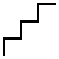
\includegraphics[valign=m]{Symbols_SVG/Steps} & 
1 & 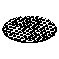
\includegraphics[valign=m]{Symbols_SVG/Surface_grain} & 
2 & 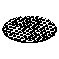
\includegraphics[valign=m]{Symbols_SVG/Surface_grain} & 
3 & 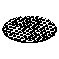
\includegraphics[valign=m]{Symbols_SVG/Surface_grain} &
4 & 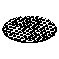
\includegraphics[valign=m]{Symbols_SVG/Surface_grain} & 
5 & 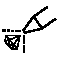
\includegraphics[valign=m]{Symbols_SVG/Lubricant_Diamond} & 
6 & 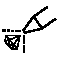
\includegraphics[valign=m]{Symbols_SVG/Lubricant_Diamond} &
7 & 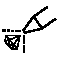
\includegraphics[valign=m]{Symbols_SVG/Lubricant_Diamond} & 
8 & 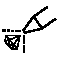
\includegraphics[valign=m]{Symbols_SVG/Lubricant_Diamond} & 
9 & 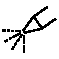
\includegraphics[valign=m]{Symbols_SVG/Lubricant_symbol}
\\ \cline{1-20} %Surfaces
Surface & 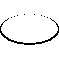
\includegraphics[valign=m]{Symbols_SVG/Surface_plain} & 
\multicolumn{2}{l|}{SiC Paper} & \multicolumn{2}{l|}{SiC Paper} & \multicolumn{2}{l|}{SiC Paper} &
\multicolumn{2}{l|}{SiC Paper} & \multicolumn{2}{l|}{MD-Dur} & \multicolumn{2}{l|}{MD-Dac} &
\multicolumn{2}{l|}{MD-Dac} & \multicolumn{2}{l|}{MD-Nap} & \multicolumn{2}{l|}{MD-Chem} 
\\ \cline{1-20} %Abrasive
Abrasive & 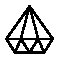
\includegraphics[valign=m]{Symbols_SVG/Diamond} & 
\multicolumn{2}{l|}{SiC} & \multicolumn{2}{l|}{SiC} & \multicolumn{2}{l|}{SiC} &
\multicolumn{2}{l|}{SiC} & \multicolumn{2}{l|}{DP} & \multicolumn{2}{l|}{DP} &
\multicolumn{2}{l|}{DP} & \multicolumn{2}{l|}{DP} & \multicolumn{2}{l|}{$\frac{1}{2}$OPS $\frac{1}{2}$Blue} 
\\ \cline{1-20} %Grit sizes
Grain Size & 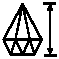
\includegraphics[valign=m]{Symbols_SVG/Diamond_Length_symbol} & 
\multicolumn{2}{l|}{P220} & \multicolumn{2}{l|}{P800} & \multicolumn{2}{l|}{P1200} &
\multicolumn{2}{l|}{P2200} & \multicolumn{2}{l|}{9$\mu m$} & \multicolumn{2}{l|}{3$\mu m$} &
\multicolumn{2}{l|}{1$\mu m$} & \multicolumn{2}{l|}{0.25$\mu m$} & \multicolumn{2}{l|}{0.04$\mu m$} 
\\ \cline{1-20} %Lubricant
Lubricant & 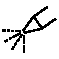
\includegraphics[valign=m]{Symbols_SVG/Lubricant_symbol} & 
\multicolumn{2}{l|}{Water} & \multicolumn{2}{l|}{Water} & \multicolumn{2}{l|}{Water} &
\multicolumn{2}{l|}{Water} & \multicolumn{2}{l|}{Blue} & \multicolumn{2}{l|}{Blue} &
\multicolumn{2}{l|}{Blue} & \multicolumn{2}{l|}{Blue} & \multicolumn{2}{l|}{Blue} 
\\ \cline{1-20} %Rotation
Rotation {[}rpm{]}& 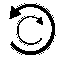
\includegraphics[valign=m]{Symbols_SVG/Rotation} & 
\multicolumn{2}{l|}{250} & \multicolumn{2}{l|}{250} & \multicolumn{2}{l|}{250} &
\multicolumn{2}{l|}{250} & \multicolumn{2}{l|}{250} & \multicolumn{2}{l|}{250} &
\multicolumn{2}{l|}{200} & \multicolumn{2}{l|}{200} & \multicolumn{2}{l|}{150} 
\\ \cline{1-20} %Force
Force {[}N{]} & 
\includegraphics[valign=m]{Symbols_SVG/Force} & 
\multicolumn{2}{l|}{30} & \multicolumn{2}{l|}{30} & \multicolumn{2}{l|}{30} &
\multicolumn{2}{l|}{30} & \multicolumn{2}{l|}{40} & \multicolumn{2}{l|}{40} &
\multicolumn{2}{l|}{40} & \multicolumn{2}{l|}{40} & \multicolumn{2}{l|}{15} 
\\ \cline{1-20} %Time
Time {[}min{]} & 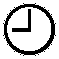
\includegraphics[valign=m]{Symbols_SVG/Clock_symbol} & 
\multicolumn{2}{l|}{until planar} & \multicolumn{2}{l|}{3} & \multicolumn{2}{l|}{3} &
\multicolumn{2}{l|}{3} & \multicolumn{2}{l|}{15} & \multicolumn{2}{l|}{5} &
\multicolumn{2}{l|}{5} & \multicolumn{2}{l|}{5} & \multicolumn{2}{l|}{10} 
\\ \cline{1-20}
\end{tabular}
\caption[Sample preparation]{Steps conducted for metallographic sample preparation for EBSD and cECCI experiments.}
\label{tab: SamplePrep}
\end{sidewaystable}
\end{document}